\chapter{Aufgabe 1: Netzwerke}

\begin{figure}[tb]
 \centering 
 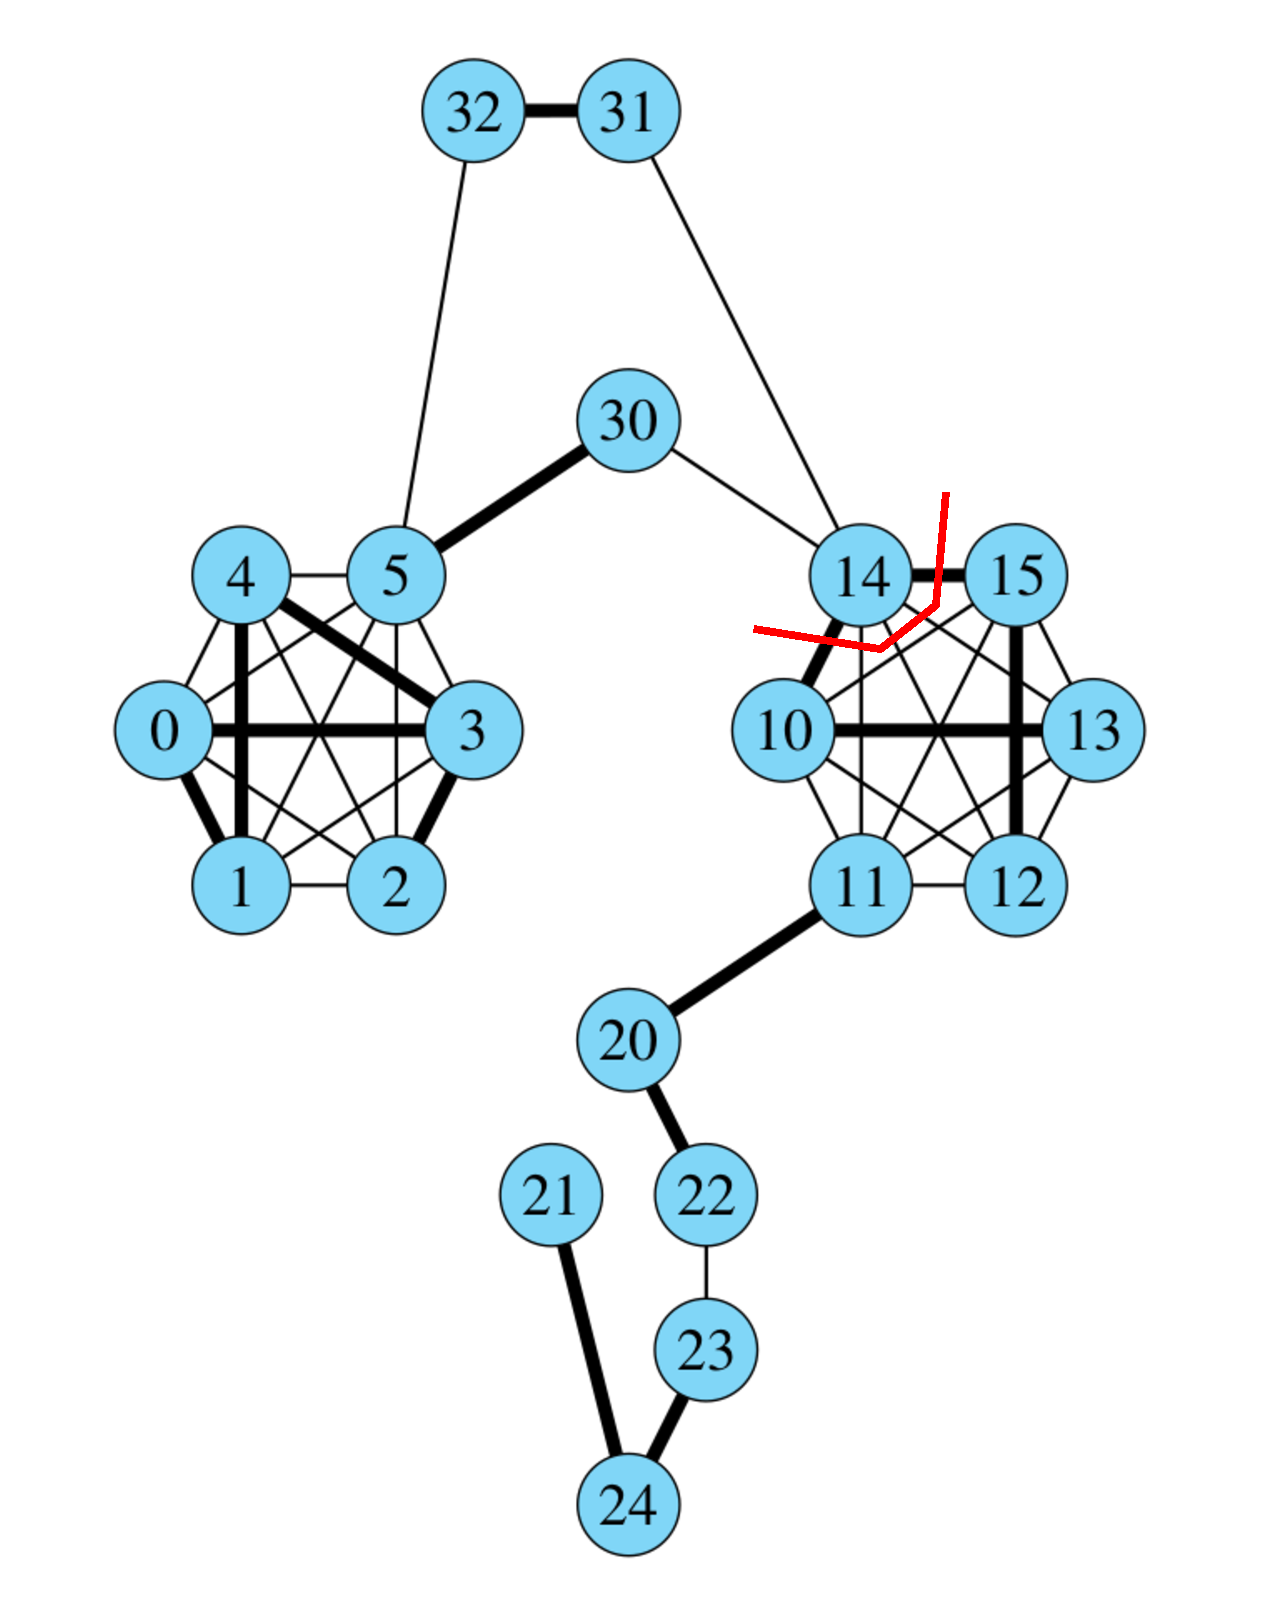
\includegraphics[width=.5\textwidth]{gegebenesNetzwerk_geschnitten.eps}
 \caption{In der Aufgabenstellung gegebenes Netzwerk. Die rote Kurve markiert den Schnitt für die Unterteilung des Netzwerks in zwei gleich große Partitionen zur Ermittlung der Bisektionsbandbreite.}
 \label{fig:netzwerk_geschnitten}
\end{figure}


\textbf{a)} Das gegebene Netzwerk weist die folgenden Netzwerkkriterien auf:
\begin{itemize}
 \item Der \emph{Diameter} bezeichnet die Kantenanzahl der größten maximalen Strecke zwischen zwei Knoten. In diesem Netzwerk beträgt der Diameter = 9 und wird verursacht durch die Strecke von Knoten 21 bis Knoten 1 über die Knoten 24, 23, 22, 20, 11, 14, 30 und 5. 
 %
 \item Teilt man das Netzwerk in zwei gleich große Partitionen hinsichtlich der Knotenzahl, sodass die aggegrierte Bandbreite zwischen ihnen -- die Summe der Bandbreiten der geschnittenen Verbindungsleitungen -- minimal wird, so bezeichnet diese aggregierte Bandbreite die \emph{Bisektionsbandbreite}. Abb.~\ref{fig:netzwerk_geschnitten} zeigt das Netzwerk und den angewandten Schnitt als rote Kurve. Dadurch entstehen zwei Partitionen mit jeweils zehn Knoten. Die Bisektionsbandbreite ergibt sich dann zu 300 Mb/s.
 %
 \item Der \emph{Netzwerkgrad} ist die maximale Anzahl der adjazenten Knoten, also der hinein- und herauslaufenden Kanten, an einem Knoten im Netzwerk. Hier beträgt der Netzwerkgrad = 7. Der verursachende Knoten ist beispielsweise Knoten 5, der Verbindungen zu den Knoten 0, 1, 2, 3, 4, 30 und 32 aufweist.
 %
 \item Die \emph{Node connectivity} bezeichnet die minimale Anzahl Knoten, die gebraucht werden, um durch deren Entfernung das Netzwerk zu unterbrechen. In diesem Netzwerk beträgt die Node Connectivity = 1 und wird beispielsweise verursacht durch die Entfernung von Knoten 20. 
\end{itemize}

\textbf{b)} Zwei Schwächen des vorgestellten Netzwerks:
\begin{enumerate}
 \item Das Netzwerk ist nicht sehr robust, da ein Knoten (Node Connectivity = 1) ausreicht, um das Netzwerk zu unterbrechen.
 \item Das Netzwerk hat teilweise sehr hohe Latenzen, insbesondere für die Knoten $20,\dots,24$, wobei der Effekt für Knoten 24 am stärksten ist (Diameter = 9). 
\end{enumerate}

\begin{figure}[tb]
 \centering 
 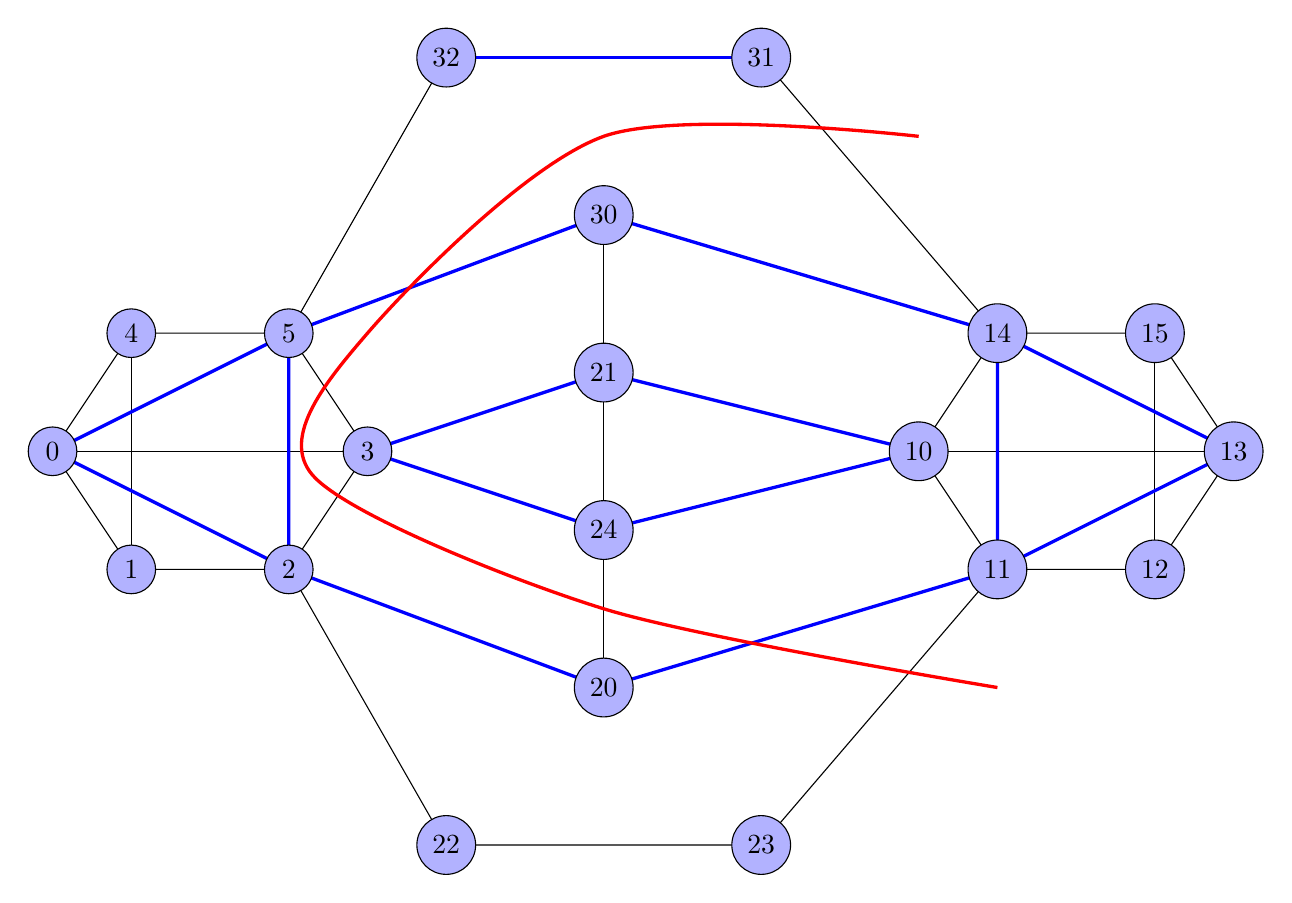
\begin{tikzpicture}
% Verbindungen
\draw (0,0) -- (1,-1.5) -- (3,-1.5) -- (4,0) -- (3,1.5) -- (1,1.5) --cycle;
\draw (1,1.5) -- (1,-1.5);
\draw (0,0) -- (4,0);
\draw[very thick,blue] (0,0) -- (3,1.5) -- (3,-1.5) --cycle;

\draw (3,1.5) -- (5,5);
\draw (3,-1.5) -- (5,-5) -- (9,-5) -- (12,-1.5);
\draw[very thick,blue] (3,1.5) -- (7,3) -- (12,1.5);
\draw[very thick,blue] (3,-1.5) -- (7,-3) -- (12,-1.5);
\draw[very thick,blue] (4,0) -- (7,1) -- (11,0);
\draw[very thick,blue] (4,0) -- (7,-1) -- (11,0);
\draw (7,3) -- (7,-3);
\draw (9,5) -- (12,1.5);
\draw[very thick,blue] (9,5) -- (5,5);

\draw (11,0) -- (12,-1.5) -- (14,-1.5) -- (15,0) -- (14,1.5) -- (12,1.5) --cycle;
\draw (14,1.5) -- (14,-1.5);
\draw (11,0) -- (15,0);
\draw[very thick,blue] (12,1.5) -- (12,-1.5) -- (15,0) --cycle;

% Schnitt
\draw[very thick,red] plot [smooth] coordinates {(11,4) (7,4) (4,1.5) (3.3,-0.3) (7,-2) (12,-3)};

% Knoten
\node[circle,draw=black,fill=blue!30!white] (0) at (0,0) {0};
\node[circle,draw=black,fill=blue!30!white] (1) at (1,-1.5) {1};
\node[circle,draw=black,fill=blue!30!white] (2) at (3,-1.5) {2};
\node[circle,draw=black,fill=blue!30!white] (3) at (4,0) {3};
\node[circle,draw=black,fill=blue!30!white] (4) at (1,1.5) {4};
\node[circle,draw=black,fill=blue!30!white] (5) at (3,1.5) {5};

\node[circle,draw=black,fill=blue!30!white] (24) at (7,-1) {24};
\node[circle,draw=black,fill=blue!30!white] (21) at (7,1) {21};
\node[circle,draw=black,fill=blue!30!white] (20) at (7,-3) {20};
\node[circle,draw=black,fill=blue!30!white] (30) at (7,3) {30};
\node[circle,draw=black,fill=blue!30!white] (22) at (5,-5) {22};
\node[circle,draw=black,fill=blue!30!white] (32) at (5,5) {32};

\node[circle,draw=black,fill=blue!30!white] (10) at (11,0) {10};
\node[circle,draw=black,fill=blue!30!white] (11) at (12,-1.5) {11};
\node[circle,draw=black,fill=blue!30!white] (12) at (14,-1.5) {12};
\node[circle,draw=black,fill=blue!30!white] (13) at (15,0) {13};
\node[circle,draw=black,fill=blue!30!white] (14) at (12,1.5) {14};
\node[circle,draw=black,fill=blue!30!white] (15) at (14,1.5) {15};

\node[circle,draw=black,fill=blue!30!white] (31) at (9,5) {31};
\node[circle,draw=black,fill=blue!30!white] (23) at (9,-5) {23};
\end{tikzpicture}
 \caption{Modifiziertes Netzwerk. Die dünnen, schwarzen Linien stellen Verbindungen mit 100 Mb/s Bandbreite, die dicken, blauen Linien stellen Verbindungen mit 1 Gb/s Bandbreite dar. Die rote Kurve markiert den Schnitt zur Unterteilung des Netzwerks in zwei gleich große Partitionen.}
 \label{fig:eigenesNetzwerk}
\end{figure}

\textbf{c)} Das modifizierte Netzwerk soll die Anzahl Knoten (20) des Originalnetzwerks beibehalten, zudem sollen die Anzahl und der Typ der Verbindungen (15 Verbindungen mit 1 Gb/s, 24 Verbindungen mit 100 Mb/s) erhalten bleiben. Der Netzwerkgrad (7) soll sich nicht erhöhen, der Diameter (9) und die Bisektionsbandbreite (2.3 Gb/s) sollen sich verbessern.

Abb.~\ref{fig:eigenesNetzwerk} zeigt unser modifiziertes Netzwerk. Im Wesentlichen wurden die Netzwerkuntergruppen mit den Knoten 0, 1, 2, 3, 4, 5 und den Knoten 10, 11, 12, 13, 14, 15 beibehalten. Ansonsten wurde Wert darauf gelegt, ein möglichst symmetrisches Netzwerk zu erstellen. Dadurch sank der Netzwerkgrad auf 6 (z.B.~verursachend durch Knoten 5 mit nur noch 6 adjazenten Knoten). Der Diameter verbesserte sich auf 5, z.B.~verursacht von der Verbindungsstrecke von Knoten 0 bis 12 über 5, 30, 14 und 13. Die Bisektionsbandbreite konnte auf 2.6 Gb/s verbessert werden, wobei Abb.~\ref{fig:eigenesNetzwerk} den gemachten Schnitt als rote Kurve zeigt, der das Netzwerk in zwei gleich große Partitionen zerlegt.